
\documentclass[paper=a4, fontsize=11pt]{scrartcl} % A4 paper and 11pt font size

\usepackage[T1]{fontenc} % Use 8-bit encoding that has 256 glyphs
\usepackage{fourier} % Use the Adobe Utopia font for the document - comment this line to return to the LaTeX default
\usepackage[english]{babel} % English language/hyphenation
\usepackage{amsmath,amsfonts,amsthm} % Math packages
\usepackage{wrapfig}
\usepackage{lipsum} % Used for inserting dummy 'Lorem ipsum' text into the template
\usepackage{tikz}
\usepackage{amsmath}
\usepackage{sectsty} % Allows customizing section commands
\allsectionsfont{\centering \normalfont\scshape} % Make all sections centered, the default font and small caps

\usepackage{fancyhdr} % Custom headers and footers
\pagestyle{fancyplain} % Makes all pages in the document conform to the custom headers and footers
\fancyhead{} % No page header - if you want one, create it in the same way as the footers below
\fancyfoot[L]{} % Empty left footer
\fancyfoot[C]{} % Empty center footer
\fancyfoot[R]{\thepage} % Page numbering for right footer
\renewcommand{\headrulewidth}{0pt} % Remove header underlines
\renewcommand{\footrulewidth}{0pt} % Remove footer underlines
\setlength{\headheight}{4pt} % Customize the height of the header
\usepackage{float}
\numberwithin{equation}{section} % Number equations within sections (i.e. 1.1, 1.2, 2.1, 2.2 instead of 1, 2, 3, 4)
\numberwithin{figure}{section} % Number figures within sections (i.e. 1.1, 1.2, 2.1, 2.2 instead of 1, 2, 3, 4)
\numberwithin{table}{section} % Number tables within sections (i.e. 1.1, 1.2, 2.1, 2.2 instead of 1, 2, 3, 4)

\setlength\parindent{0pt} % Removes all indentation from paragraphs - comment this line for an assignment with lots of text

%----------------------------------------------------------------------------------------
%	TITLE SECTION
%----------------------------------------------------------------------------------------

\newcommand{\horrule}[1]{\rule{\linewidth}{#1}} % Create horizontal rule command with 1 argument of height

\title{	
\normalfont \normalsize  % Your university, school and/or department name(s)
\horrule{0.5pt} \\[0.4cm] % Thin top horizontal rule
\huge Physics 422 H.W. 1\\ % The assignment title
\horrule{2pt} \\[0.5cm] % Thick bottom horizontal rule
}

\author{Josh Lucas} % Your name

\date{\normalsize\today} % Today's date or a custom date

\begin{document}

\maketitle % Print the title

%----------------------------------------------------------------------------------------
%	PROBLEM 1
%----------------------------------------------------------------------------------------

\section{Lattice Planes}
\textbf{Draw a series of cubic unit cells with the following lattice planes on them}\\
$\bullet$ (001), (110), (201), (2$\bar{1}$0), (1$\bar{1}$1)
\begin{figure}[!h]
\includegraphics[width = \linewidth]{sec1}
\caption{Miller indices from left to right; (001), (110), (201), (2$\bar{1}$0), and (1$\bar{1}$1) }
\end{figure}
%
%\begin{figure}[!htb]
%\minipage{0.19\textwidth}
%  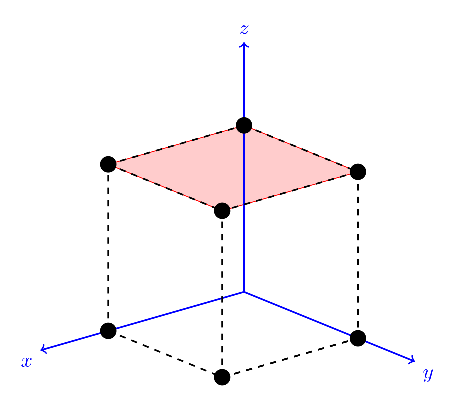
\includegraphics[width=1.2\linewidth]{001}
%\caption{(0,0,1)}
%\endminipage\hfill
%\minipage{0.19\textwidth}
%  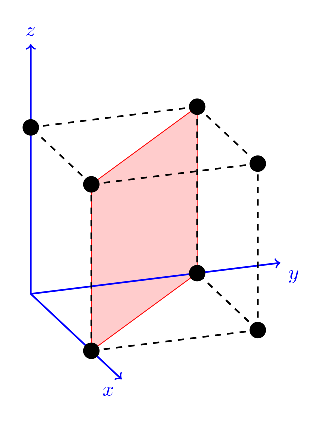
\includegraphics[width=.8\linewidth]{110}
%  \caption{110}
%\endminipage\hfill
%\minipage{0.19\textwidth}%
%  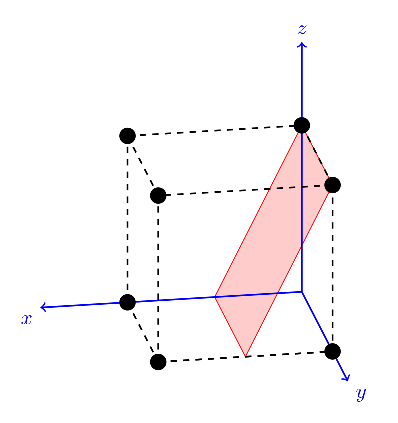
\includegraphics[width=\linewidth]{201}
%  \caption{2,0,1}
%\endminipage
%\minipage{0.19\textwidth}
%  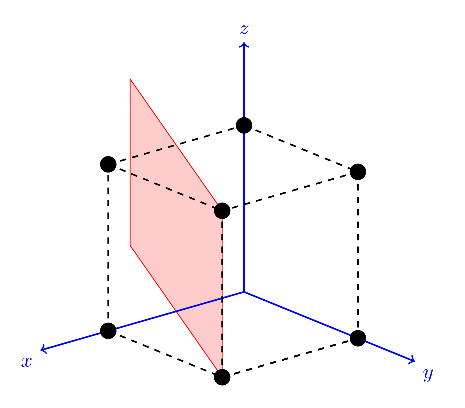
\includegraphics[width=1.2\linewidth]{2-10}
%\caption{(2,-1,0)}
%\endminipage\hfill
%\hspace{4mm}
%\minipage{0.19\textwidth}
%  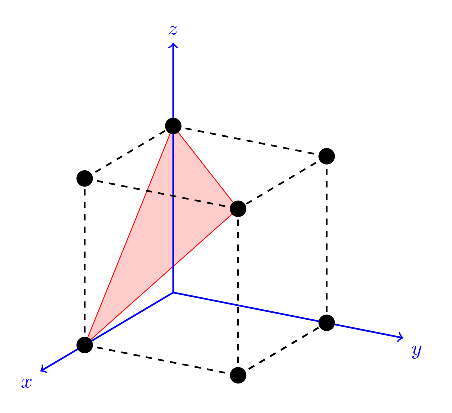
\includegraphics[width=.8\linewidth]{1-11}
%  \caption{(1,-1,1)}
%\endminipage\hfill
%\end{figure}









%----------------------------------------------------------------------------------------

\end{document}